\documentclass{article}

\usepackage{pgf}
\usepackage{tikz}
\usetikzlibrary{arrows,automata}
\usepackage[latin1]{inputenc}
\usepackage{verbatim}

\begin{document}

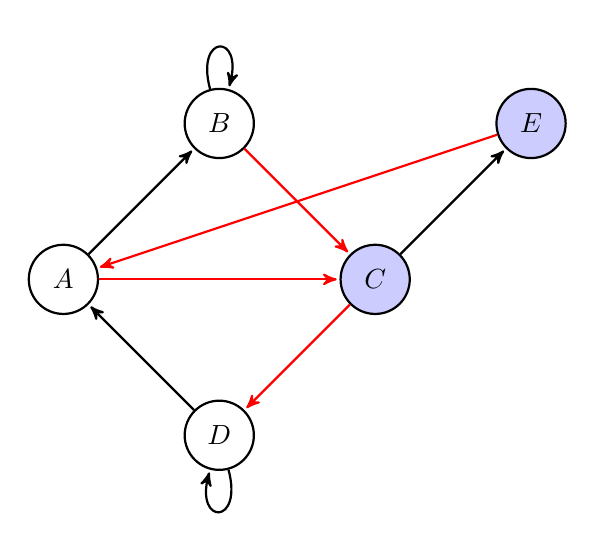
\begin{tikzpicture}[->,>=stealth',shorten >=1pt,auto,node distance=2.8cm,
                    thick]

  \node[state] (A)                    {$A$};
  \node[state] (B) [above right of=A] {$B$};
  \node[state] (D) [below right of=A] {$D$};
  \node[state, fill=blue!20] (C) [below right of=B] {$C$};
  \node[state, fill=blue!20] (E) [above right of=C] {$E$};

  \path (A) edge [] node {} (B)
            edge [red] node {} (C)
        (B) edge [loop above] node {} (B)
            edge [red] node {} (C)
        (C) edge [red] node {} (D)
            edge node {} (E)
        (D) edge [loop below] node {} (D)
            edge node {} (A)
        (E) edge [red]  node {} (A);
\end{tikzpicture}

\end{document}
